
\begin{savequote}[8cm]

    We hear a lot these days about genes and molecules, but how does one human brain, or one human being coordinate, or entrain, or resonate with another?  We may not realise it but we live in a world of coordination, at every level and every scale of endeavour.

  \qauthor{--- J. A. S. Kelso  \textit{Coordination and the Complimentary Nature} Presentation to the The New York Academy of Sciences - May 12, 2010}
\end{savequote}


%I do not see any way to avoid the problem of coordination and still understand the physical basis of life.
%\qauthor{--- H. H. Pattee  \textit{The role of instabilities in the evolution of control hierarchies} 1976}


\chapter{\label{chap:theory}A theory of social bonding through joint action}


\minitoc

%In response to the knowledge gaps identified in the Introduction, in this chapter I outline a novel theory of social bonding through joint action, which will be tested in subsequent empirical studies of joint action among Chinese rugby players.  While it is now well-established that successful interpersonal entrainment of movement can be responsible for generate positive psychological and social effects, the mechanisms through which entrainment is achieved remain poorly understood.  In particular, I identify team click as a special case phenomenon of joint action and a potential mediator of the relationship between joint action and social bonding in group exercise contexts.  Emerging research from the social cognition of joint action suggests that a continuum of cognitive mechanisms are responsible for establishing and maintaining behavioural coordination between two or more individuals.  More efficient solutions to the cognitive uncertainty of joint action appear to involve reducing the cognitive demands associated with interoceptive predictive modelling and instead increasing reliance on more direct extra-neural coupling with the environment.  These mechanisms also appear to be modulated by inter-individual and cultural variation in knowledge, expertise, experience, and personality type.  Evidence suggests coordination in joint action can set the foundation for social connection, and the phenomenon of team click can be understood as an optimal state of interpersonal coordination in joint action that maximally activates a causal pathway between joint action and social bonding.  I conclude the chapter by summarising a theory of social bonding through joint action, and outlining predictions that arise from this theory.

%In this dissertation I attend specifically to the relationship between joint action and social bonding in the group exercise context of professional rugby in China.  In this chapter I formulate a novel theory of social bonding through joint action in order to address the knowledge gaps in the social high theory of group exercise and social bonding.


                                  \begin{CJK}{UTF8}{gbsn}

\section{The development of visceral agency in rugby's newest recruit\label{sect:SHW}}
Sun Hongwei arrived, escorted by his high school athletics coach, to the Beijing Temple of God of Agriculture Institute of Sport (hereafter the Institute) soon after I began my fieldwork in August 2015.  An 18-year-old with a slight build and timid demeanour---his gaze remained diverted to the ground during his first few months at the Institute---Hongwei later told me that he had never seen a rugby ball before that day he arrived.

Hongwei was from Hebei province, immediately surrounding the special prefecture of Beijing, China's capital.  Hongwei's coach had organised a trial for Hongwei with the Beijing Provincial men’s and women's Rugby Program (hereafter the Program) by calling upon social connections to the leadership of the Institute.  Athletes come to the Rugby Program from all over the country.  As I explain in more detail in Chapter ~\ref{chap:researchSetting}, representing Beijing at a provincial level in a sport like rugby can translate into the opportunity to gain entrance to one of China's top universities and enhanced career employment opportunities thereafter.

Rugby is not a popular sport in China, but its recent inclusion in the Olympic games (in the form of the modified seven-a-side version of ``rugby sevens'') means that it now occupies a prominent place in the Chinese sport system.  Rugby programs such as the one at the Institute now exist in 12 of China's 34 provincial level regions, either embedded within, or somehow associated with, tertiary education institutions.  Thus, although rugby and China are not commonly associated terms, rugby now affords Chinese athletes a rare and under-capitalised opportunity to pursue attractive life-course opportunities of education and employment in an intensely competitive education system.

Without exception, the athletes who arrive at the Institute to join the rugby team were not like me; they had not spent their childhoods playing rugby in their schoolyards or watching professional rugby on television. Many who come to rugby transition from other more popular sports such as athletics, basketball, or association football, and often---like Hongwei---have never seen a rugby ball before they arrive.  Most ``start from scratch,'' so to speak, in terms of their grasp of the requirements of the highly interactive and technically complex team sport. In addition to complex patterns of movement coordination, rugby also involves unrestrained body-on-body collisions and intense bouts of high physiological exertion, requiring speed, strength, agility, and endurance to perform all of rugby's technical requirements successfully (see Chapter ~\ref{chap:researchSetting} Section ~\ref{sect:rugbyUnion}).  Learning the game of rugby from a baseline of essentially zero, while also navigating the inevitably demanding social and political dynamics within the team and the Institute, was clearly going to be a daunting task for Hongwei.


                        \begin{center}
                          * * *
                        \end{center}

Hongwei was the first of the Program’s new recruits that I followed closely.  Even compared to other newly arrived junior athletes, he was noticeably timid and shy, particularly in his interactions with the coaches (myself included) and senior players. Nevertheless, Hongwei clearly signalled diligence and commitment through his participation in team activities.  He arrived early to each training session, and carried more than his fair share of the training equipment---a task shared by the most junior members of the team.  Each time I passed Hongwei in the corridors of the Institute he would greet me with a polite bow and greeting, ``Hello Coach'' (\textit{'jiaolian hao'} `教练好').  In these instances, Hongwei would coordinate his greeting with a moment's eye contact, only to return his gaze to the floor and continue walking.

Due to his lack of familiarity with the basic techniques of rugby, Hongwei was initially unable to fully participate in normal training with the rest of the team.  Instead, during the first month or so, Hongwei stood on the sidelines and practiced the basics with other athletes who were unable to fully participate in training due to injury.  He learning how to pass and catch the rugby ball, while stationary and running in-motion.  In my eyes at least---eyes of an observer accustomed to instinctual grasp of these movements from a young age---Hongwei's attempts to accustom himself with the skills of rugby were jarring.  The idiosyncrasies of rugby's ovular ball often foiled him.  I would regularly see him chasing after a ball on the ground he'd just fumbled, as if he was chasing in vein after a scurrying rabbit tactfully evading its pursuer.

                        \begin{center}
                          * * *
                        \end{center}

I interviewed Hongwei approximately six weeks after he arrived at the Institute.  Hongwei's demeanour during the interview was consistent with the timid and shy one that he presented publicly at training.  As explain below, he did show some signs of captivation with his new sport and social environment.  When I asked about his initial impressions of the on-field demands of rugby, however, Hongwei was quick to confess that he felt utterly unacquainted:

  \begin{quote}
    SHW: I still haven’t really started to practice any of the team plays or anything; all I can do so far is pass and run a little bit...(but) it's quite fun! \\
    JT: What do you think is the most difficult component of rugby? \\
    SHW: Um\textellipsis well, coordinating with teammates [on the field], particularly coordination in attack.  Because I can't figure it out.  When I first arrived, I didn’t even know what a ``switch play'' or a ``blocker play'' was.
  \end{quote}

  \begin{quote}
    SHW: 战术没怎么接触,就是像传球啊、跑动什么的会一点了 \\
    JT: 感觉怎么样?\\
    SHW: 挺好玩的!\\
    JT: 你认为橄榄球最难的一部分是什么? \\
    SHW: ...打配合,进攻的配合,因为搞不明白,刚来的时候也不知道什么交叉,后插什么的 \\
  \end{quote}

Hongwei was self-critical in this confession regarding his minimal grasp of the technical requirements of joint action in rugby.  The obvious stress and anxiety he expressed was indicative of a broader trend with the other athletes I interviewed, as I will explain in more detail in the ethnographic sections of this dissertation (see Chapters ~\ref{chap:ethnoField} \nobreakdash~\ref{chap:ethnoResults}). When athletes were asked in interviews about the most difficult aspect of rugby, on-field coordination with teammates was by far the most common answer, particularly among the new recruits and most junior athletes.

As I directed the interview towards topics beyond the on-field technical demands of rugby, Hongwei was more positive, framing rugby as an exciting new opportunity, and commenting that his friends and family were in awe of the fact that he is playing such an impressively ``strong'' physical sport like rugby.  When I asked him about something new that he had learnt through playing rugby, Hongwei automatically responded by emphasising the social dimensions to his experience at the Institute:

  \begin{quote}
    ``...I think it's mainly this thing of having teammates. Before, when I was training for an individual sport, it was just me training by myself. [In that environment] it was a case of whoever trained well was successful.  But now with this team of brothers, elder teammates will take care of younger teammates. We all train together, and if you can’t do something, you can always ask your elder teammates...[Rugby] is so much better, because in an individual sport, if you can't master something, you have to go to your coach for help. Other athletes don't want to teach you, because if you surpass them, then they have to work even harder to keep up... I have had to learn about helping others, because rugby is not like an individual sport, where you look after your own performance and that's it.  In a team sport, if you don't do well, there's no need to get too frustrated or upset, because other athletes will help you out, and I will also help others out, that type of collaboration with each other.''
  \end{quote}

\begin{CJK}{UTF8}{gbsn}
  \begin{quote}
    我觉得主要是师哥师弟的这一块儿,原来练个体项目都是自己练自己的,谁练好了谁厉害,但是现在师哥师弟,有师哥照顾师弟带着,互相练,我不会我可以问师哥
    ...因为个人项目你不会就必须要找教练,但是别人不愿意教你,因为你把别人超越了那别人还还得努力。 学到互相帮助,因为向个体项目自己成绩自己来拿就行,而像团体项目,即使自己做不好,也不用太泄气太沮丧,因为别人会帮你做好,我也会帮别人做好,互相协作的那种.
  \end{quote}
\end{CJK}

Hongwei's explicit reference to the collegiality of the team, and his position as junior member, highlights that the technical skills of rugby were not the only novel components of his experience.  Hongwei's background was in track and field (his event was pentathlon, very much an individual sport), and the team environment was completely new to him.  This was also the case for many of the other athletes in the team.  As I listened to his experiences associating rugby and group membership, I could not help but associate the quality of these declarations of prosociality with his overly mechanical imitation of rugby's foundational techniques.  In both I saw his willingness and desire to signal commitment; but both lacked a certain grasp or command that one would expect from an athlete more habituated to rugby.

                            \begin{center}
                              * * *
                            \end{center}

A few months passed, and Hongwei continued to train.  He was as eager and committed as when he began, and I did notice some gradual improvement in his grasp of rugby's basic skills.  But he also remained extremely reserved, keeping his head low at all times in team settings, unless addressed by senior players or coaches.

Then, one evening when I had returned to my room in the Institute dormitory from a three-week hiatus in Australia over Christmas of 2015, I heard a knock on my open door, and to my surprise Hongwei took an assertive stride into my room, carrying in two arms a draw-string bag containing rugby balls (which were in need of more air before the next day's training session).  Hongwei had never ventured into my room before, apart from our first interview two months earlier---but certainly never on his own accord.  Remarkably, Hongwei looked me straight in the eyes with his head held high and energy beaming from his face and chest.  I couldn't help but smile and ask, with genuine intrigue, ``How have you found training recently?''
``Very good'' he said, assertively and excitedly.  ``Much better than before.  At least now I know what’s going on at training, I can keep up with the plays!''  A big smile grew on his face as he continued to hold my gaze.  ``Oh good!'' I said, a little bit shocked.  I congratulated him for his hard work in training while I had been away, and encouraged him to keep at it.  Wow, I remember thinking to myself, Hongwei was all of a sudden possessed by a powerful force.  Somehow, his adherence to rugby had instiled him with a visceral sense of agency.

                          \begin{center}
                            * * *
                          \end{center}

In the same way that Adrian's opening monologue (Chapter ~\ref{chap:intro} Section ~\ref{sect:adrian}) suggested a relationship between the on-field dimensions of rugby and social processes between teammates, the fact that aspects of Hongwei's personal and social demeanour at the Institute appeared to covary with his familiarity with the technical requirements of rugby over time suggests a relationship between joint action and group membership that is worthy of further investigation.
%HW's change is a change in attitude (Bateson) agency

How is it possible to scientifically account for the unmistakably ``visceral'' quality of Hongwei's transformation from timid newcomer to budding Beijing rugby player?  How can these ethnographic observations be explained in terms of generalisable cognitive mechanisms and systems dynamics of joint action?  Finally, and ultimately, how do answers to these questions improve our ability to comprehend the evolutionary significance of group exercise in the human record?



\section{The need for a theory of joint action and social bonding in group exercise}
As the story of SHW anecdotally suggests, the visceral dimension of group exercise may take time to develop.  Presumably in  Adrian I witnessed the finished product: through many years of on- and off-field engagement with the sport of rugby, Adrian came to embody rugby and its carnal mystery.  When I met him during my first stint of research at the Institute, Sun Hongwei was only just beginning this journey. As explained in the previous chapter, a theory that can account for the dynamic and interlocking physical, cognitive and social dimensions of group exercise is yet to be fully formulated.  In this chapter, I propose that a novel theory of social bonding through joint action can shed light on the on the scientific mechanisms underlying this hitherto mysterious phenomenon.

The novel theory proposed in this chapter builds upon the hypothesis that group exercise is causally relevant to processes of social cohesion \citep{Dunbar2010,Whitehouse2014,Cohen2017}.  Empirical research programs within cognitive and evolutionary anthropology have begun to draw attention not only to the “cognitive” dimensions of human behaviour, sociality, and cultural evolution (as they are narrowly defined by traditional “stimulus-reponse” models \citep[][]{Marr1985}).  In addition, researchers identify the role of physiological and affective mechanisms of neurobiological reward and autonomic arousal in supporting human cognition and evolution.  As Dunbar and Shultz suggest, it is impossible to accept that humans adhere to a ``dung fly'' model of mere (social) aggregation; it is clear that humans have evolved a species-unique tendency to actively congregate and cohere around shared cultural practices \citep[cf.][]{Tomasello2005}.

But, as explained in the introduction, existing approaches to the empirical question of human bondedness and social cohesion are marred by a commitment to a model of cognition in which physicality, information, and culture are examined as conceptually and causally distinct processes.  As a result, the social high theory of group exercise and social bonding \citep[cf.][]{Cohen2017} lacks an account of how extreme physiological cost generates profound meaning, or how cognitive complexity in joint action (beyond strict behavioural synchrony) can produce autotelic experiences of flow and team click, with flow on social effects (see Chapter ~\ref{chap:intro} Sections ~\ref{sect:}\nobreakdash~\ref{sect:}.  The modes theory \citep[cf.][]{Whitehouse2004} proposes a causal link between physiological cost (arousal) and a high quality manifestation of social bonding mediated by rich processes of social identity and meaning (identity fusion). This link sits at one end of a bi-modal distribution of ritual practices, the other end being a link between ritual memorability (cognitive complexity) and semantically-mediated social identification.  While these two modes of ritual practice and social cohesion are deliberately cast as theoretical extremes, to date there have been very few productive attempts to verify the gradient in between.  Meanwhile, models od cultural evoluitonary that underpin these approaches to social cohesion remain entrenched in empirical debates that revolve around the proximate mechanisms of transmission of densely semantic cultural variants (i.e. representations), despite best efforts to theorise a fuller spectrum of interlocking physiological, cognitive, ecological, and social ``factors of attraction.''  In this dissertation, I propose that a more dynamical and integrative model of cognition is needed in order to make empirical progress on the question of the role of group exercise in human sociality, and indeed scientific questions relating to behaviour and evolution more broadly.

More so than most cultural variants that have traditionally formed the focus of scientific analysis, activities in which group exercise feature demand a dynamic conception of cognition.  Group exercise invariably involves brains and bodies engaged in “in-the-moment” and “on-line” coordination of action (joint action).  From a pure computational perspective, achieving and sustaining joint action is a daunting cognitive task, as it requires the coupling and constraining of the various degrees of freedom of autonomous co-actors \citep{Bernstein1967}.  However, it is now more clearly understood that human cognition—and indeed, cognition of biological life more generally—does not rely on pure, “brute-force” computation, like that of digital computers, to manage to the challenges of interacting with the environment, particularly with others \citep{Yufik2013}.  Rather, prevailing theories of cognition suggest that humans flexibly deploy a range of strategies in order to anticipate and regulate the uncertainty inherent in joint action.

In fact, one of the core cognitive strategies that has been overlooked by traditional ‘’stimulus-repsonse” models of cognition (which were inspired originally by digital computers) is action itself.  The integration of movement into human inference through the “Active Inference Framework \citep[hereafter ‘’AIF’' cf.][]{Friston2010} promises a clearer theoretical framework within which to conduct empirical research of observable human behavioural and evolutionary phenomena \citep{Clark2015,Linson2018}.  Specifically, and for the purposes of this dissertation,  AIF enables predictions for how humans click, connect, and cohere through joint action typical of group exercise contexts.

In this chapter, I develop testable predictions for a relationship between joint action and social bonding.  I theorise team click as a psychological construct that mediates a relationship between joint action and social bonding.  While the social relevance of team click and the related concept of flow have evaded rigorous analysis using traditional theories of cognition—due in most part to the limitations of these traditional theories \cite{Dietrich2004,Slingerland2014}—within the AIF, team click can be theorised as a special case in which the bonding effects of joint action are maximised.

Preview theory here:
As I outline in full detail in the sections below, a theory of social bonding through joint action depicts two or more brains

In the sections that follow, I first introduce the cognitive challenge of joint action and the phenomenon of team click and explain its suitability as a real-world empirical anchor and novel psychological construct for a novel theory of social bonding through joint action (Section ~\ref{sect:dfProblem}).  I then introduce the AIF, including its three core tenets of thermodynamic cognition, predictive coding, and (cultural) affordances (Sections ~\ref{sect:}\nobreakdash~\ref{sect:}).  With this grounding, I review attempts to apply AIF to joint action, and explain how mechanisms responsible for blurring of self and other agency, affective reward, and shared attention could give rise to experiences of team click and social bonding through joint action (Section ~\ref{sect:}).  I then outline the application of AIF to group exercise in particular, explaining how group exercise environments are rigged to produce extreme levels of cognitive uncertainty, while also making available social and cultural affordances capable of attenuating uncertainty (Section ~\ref{}).  Finally, I present a novel theory of social bonding through joint action, and outline general predictions that emerge from this theory.


\subsection{Introducing the phenomenon of team click\label{sect:teamClickIntro}}

In this section I outline the phenomenon of team click, and point to evidence of its connection to mechanisms of joint action and social bonding.

One of the big mysteries of competitive team sport, particularly at the elite level, is the elusiveness of peak team performance.  While each individual athlete may exhibit expert level competence in sport specific skills, the much sought after aggregation of these components, i.e., a team that consistently performs ``in the zone,'' and ``firing on all cylinders,'' in reality often proves frustratingly difficult to achieve and sustain.  As King and De Rond \textcite[568]{King2011} note in their ethnography of the 2008 Cambridge University rowing crew who participated (and who were eventually victorious) in the famous annual Boat Race against Oxford University, the search for collective rhythm is a universal in human social interaction, but  the physiological and psychological complexity of finding that rhythm ``...is extremely difficult to attain; collective performance is a possibility not a certainty.''   The moment in which everything ``clicks'' into place in team sport can, for various reasons, disappear as abruptly as it arrives, if indeed it arrives at all.

But, when team click is somehow cultivated, and even sustained, it is celebrated as the ultimate, albeit often inexplicable magic of sporting feats. Consider Leicester City Football Club's unbelievable outhouse-to-penthouse title run in the 2015 English Premier League, the recent dominance of the Golden State Warriors in the American National Basketball League, or the astonishingly consistent performance of the New Zealand men's national rugby union team (the ``All Blacks'').
    \footnote{The All Blacks are arguably the most successful sporting team ever, with a winning percentage of 77\% in the last 150 years (and 88\% in the last 6 years) \citep{Kerr2013}.}
All of these successful teams carry with them a powerful ``aura'' associated with their capacity to effectively coordinate their behaviours on the field over extended time scales: individual games, seasons, and, in the case of the All Blacks, entire generations.  The aura associated with such rare instances of collective performance can seduce fascination and elaborate exegesis.

    %In this thesis I commit to the more banal task of naturalising the phenomenon of team click, by locating it within a novel theory of social bonding through joint action.

For the purposes of this dissertation, I use the term team click to describe the phenomenology of peak performance within a team of athletes engaged in joint action, but the term has potentially broader applications beyond group exercise.  For athletes, coaches, and spectators alike, team click can be a hugely powerful sensation.  As theologian Michael Novak explains, ``[f]or those who have participated on a team that has known the click of communality, the experience is unforgettable, like that of having attained, for a while at least, a higher level of existence'' \citep[11]{White2011}.  As explained int he previous chapter (Chapter ~\ref{chap:intro} Section ~\ref{sect:linksComplexClick}), the experience of optimal performance in sport has been extensively documented in the psychological literature of flow \citep{Csikszentmihalyi1992,Jackson1995,Jackson1999,McNeill1995}.

Psychologists and neuroscientists have extensively studied the experience of flow, and have tabled a series of neuropharmacological \citep{Boecker2008}, neurocognitive \citep{Dietrich2006,Dietrich2011,Labelle2013}, and psychological \citep{Csikszentmihalyi1992} theories for its emergence.  The vast majority of flow research has focussed on the experience of the individual---the athlete, musician, or performer.  Some attempts have been made to extended an analysis of flow and its antecedents to the level of the group and dynamics of interpersonal coordination---a phenomenon termed ``group flow'' \citep{Sawyer2006}---but these attempts lack coherence and development.  Anecdote and observational evidence suggests that in addition to the components of flow already identified at the level of the individual, successful performance of technically complex
\textit{joint} action (beyond exact in-phase synchrony) could have distinct psychological and social consequences.




    %The experience of flow has by now been extensively studied by psychologists and neuroscientists, from which a series of neuropharmacological \citep{Boecker2008}, neurocognitive \citep{Dietrich2006,Dietrich2011,Labelle2013}, and psychological \citep{Csikszentmihalyi1992} theories for its emergence have been tabled.  The vast majority of flow research has focussed on the experience of the individual---the athlete, musician, or performer.  Some attempts have been made to extended an analysis of flow and its antecedents to the level of the group and dynamics of interpersonal coordination---a phenomenon termed ``group flow'' \citep{Sawyer2006}---but these attempts lack coherence and development.

  Team click shares many similarities with the psychological states associated with flow, but is distinct in that it specifically delineates perceptions of joint action from individual action, and therefore implicates physiological, cognitive, and social mechanisms unique to joint action \citep{Vesper2010}, including the complexity systems dynamics associated with participating in a socially-coordinated, multi-agent system of physical movement \citep{Kelso2009}.  Team click is anecdotally present in a wide range of joint action contexts, and is often associated in these contexts with psychological processes of positive affect and wellbeing, as well as personal agency, social affiliation, and group membership \citep{Jackson1995,Marsh2009,Wheatley2012,Slingerland2014}.


  The experience of team click, like flow, also often involves positive violations of individual expectations about action.  While elite athletes presumably always aim for optimal joint action, the experience of actually achieving that desired state, and even exceeding it---often with the help fo co-actors---appears to be a powerful, and somewhat ``surprising'' experience.  In the 1990s, psychologist Susan Jackson conducted a number of qualitative studies documenting athletes' (in this case elite figure skaters) experience of flow in solo and joint action

    \begin{quote}
      Oh, it's awesome! Everything's at peace...the crowd was involved, we were involved as a pair team, and we were just aware of everything, it just kept snowballing, like we weren’t going to miss, and it was great, it was an awesome experience \citep[168]{Jackson1992}.
    \end{quote}

Here, the athlete to have been in awe of his or her own performance.  Part of the awesomeness may derive from the rare feeling of absolute alignment between self and co-actor(s):

    \begin{quote}
      What was really so special about this performance was that there was nothing between (partner's name) and I but flow.  You know, through the whole three minutes.  That meant that her mind and my mind were clear and in the same...in a partnership. It's always adjustments for ``Am I?'' and ``Are You?'' and ``Where Are We?'' and stuff like that.  That day was really a marriage of (partner) and (self) and the ice.  So I think it's a different kind of flow experience than a single skater who has much more control over themselves. \citep[173-4]{Jackson1992}.
    \end{quote}

This passage, taken from an interview with a professional figure skater, demonstrates the key elements of distinction between the experience of click in solo and joint action. As I will explain in more detail below, joint action requires constant finessing (adjustments) of behaviours and intentions between co-participants in which individuals are consulting internal models of self, other, and joint action \citep{Pesquita2017}.  This passage highlights the cognitive complexity of joint over individual action, suggesting the cost and uncertainty associated with attending to and attempting to control the movement degrees of freedom of others in addition to one's own.  The achievement of ``click'' in joint action may instead represent a jitter-less ``co-confidence'' \citep{Noy2015,Noy2017}, in which fixation on the contributions of ``you'' and ``I'' are momentarily abandoned or down regulated, and the agency of ``we'' is realised \citep{Gallotti2013,Friston2015}.

Importantly, team click appears to have important flow-on consequences relevant to social bonding and affiliation. Tightly synchronised activity in particular, found in team sports such as rowing, can help dissolve the boundaries between individual and social agency: ``In rowing...it feels like you have at your command the power of everybody else in the boat. You are exponentially magnified. What was a strain before becomes easier. It is absolutely the ultimate team sport'' \citep[x]{Brown2016}.
The blurring of agency between self and team may be responsible for facilitating affiliation and trust between teammates in competitive athletic environments such as professional rugby, which often involves high physiological stress and uncertainty.  As Jeremy Paul, a famous Australian Rugby player commented of his late teammate, Dan Vickerman: ``...you always wanted a guy who would go into the trenches with you and he always played consistently well...he could really play and was just one of the good lads that you enjoyed his company'' \citep{Fox-Sports2017}.  In this sense, the experience of team click may act as a social diagnostic tool, a powerful signal of commitment to joint action and willingness to cooperate \citep{Reddish2013a}. \\

Team click refers to the perception of peak team performance.  Based on anecdote and evidence from psychology and anthropology, an individual's perception of team click should contain some or all of the components outlined in Figure ~\ref{fig:clickComponents}.


        \begin{figure}
          \noindent\fbox{%
              \parbox{\textwidth}{%
              \\        \begin{enumerate}
                        \item Flow or coherence of joint action
                        \item Tacit understanding between co-actors
                          \begin{enumerate}
                            \item Perceived reliability of self and co-actor
                          \end{enumerate}
                        \item Atmosphere or aura around team performance
                        \item Blurring of the boundaries between individual and team /teammate agency
                          \begin{enumerate}
                            \item Others are responsible for extending individual ability
                          \end{enumerate}
                      \end{enumerate}
                      }%
                  }
              \\
          \caption{Components of team click}
          \label{fig:clickComponents}
        \end{figure}


    \\
    \\
    \\
  As explained above, team click is a phenomenon distinct to joint action.  Team click involves an experience of pleasurable flow or coherence of joint action, tacit (rather than explicit) understanding between co-participants, a degree of aura or atmosphere around joint action, a blurring of agency between self and teammates or group (or ``we''), and perception of reliability of others and self in performing their roles.  Team click offers a powerful empirical anchor for exploring a broader relationship between joint action and social bonding in group exercise contexts.  In the sections that follow, I outline the building blocks necessary to formulate a novel theory of social bonding through joint action.  Within this theory, team click is proposed as a mediating construct, through which the bonding effects of joint action are maximised.

Researchers have pointed out that flow---a concept that shares many similarities with team click---has traditionally escaped rigorous scientific analysis \citep{Dietrich2010a,Slingerland2014}.  Dietrich, for example, explains that flow presents a paradox that is difficult to explain according to traditional theories of attention and mental effort, which tend to assume better performance, on any task, is associated with increased conscious effort allocated to that task \citep{Dietrich2004b}.  Flow appears to entail spectrum of both effortful (intentional, mental) and seemingly effortless cognitions implicating embodied action and the resources of the bio-external environment.  Team click, too, is a multidimensional process involving mental, embodied, emotional, and social dimensions.


\section{Human solutions to the challenge of joint action\label{sect:dfProblem}}
%\subsection{The degrees of freedom problem and its solutions in human movement}

\textcite{Bernstein1967} was the first to point out the astounding computational challenge associated with coordinated physical movement in multi-component living systems.  In the case of human intra-personal movement, for example, an impressive balance is somehow struct between flexibility, precision, and control, whereby hundreds of muscles and joints coordinate to perform many different tasks of everyday life.  When we grasp a cup or catch a ball, many individual muscles and joints---each with their degrees of freedom---work together in fine concert.  Bernstein found it unlikely, from a computational perspective, that the central nervous system would be able to finely control all the possible movements (the degrees of freedom) of each single muscle individually to create coherently directed movements---it would be computationally impossible.  Rather, he suggested that muscles and joints form  ``functional synergies''---flexible function-specific self-organising assemblies---by locally coupling and constraining each other’s degrees of freedom to greatly reduce the amount of control needed.

Intra-personal and interpersonal human movement both rely on the nervous system’s capacity to anticipate, attend, and adapt to the conditions of the environment \citep{Keller2014}.  In the case of intra-personal human movement, successful coordination of is made possible by the nervous system's direct access to information concerning the spatiotemporal position of the body and its relationship to the environment.  Privileged access to this information enables habituated coupling of movement control system to the organism's various degrees of freedom, and therefore the emergence of self-organisng functional synergies.

By contrast, interpersonal movement coordination poses a much more significant challenge.  In the case of interpersonal coordination, the combination of 1) limited reliability of sensory modalities as a source of information about the action of others \citep{Wilson2005,Wolpert2003,Frith2007} and 2) the informational complexity associated with a cognitive system comprising multiple autonomous agents \citep{Bernstein1967} means that successful coordination in joint action is an inherently difficult and highly improbable cognitive challenge.  How exactly do humans face up to this cognitive challenge, and, quite often, successfully surmount it?

An answer to this question requires close attention to the various sophisticated cognitive, behavioural, and cultural capacities that define human's species-unique evolutionary niche \citep{Roepstorff2010,Clark2015,Fuentes2016}. Our ability for technical manipulation of extra-somatic materials and ecologies; advanced theory of mind; and information-rich, malleable, and scalable communication systems affords complex behavioural repertoires involving that enable interaction between groups as small as two and conceivably as large as two million \citep{Nowak2017}.  In this dissertation I focus on interpersonal coordination of physical movement as a basal layer to human social interaction that facilitates the subsequent coordination of many towering layers of informational complexity.

\textcite{Vesper2010}, building on previous work by  \textcite{Sebanz2006}, have proposed a minimal architecture for joint action.  The minimal architecture of joint action requires that individuals:

\begin{enumerate}
  \item Represent a shared goal, as well as representing one’s own individual contribution to the shared goal.
  \item Apply monitoring and prediction processes to each partner’s actions. This includes monitoring the extent to which shared goals or tasks are being fulfilled while at the same time predicting a partner’s actions.
  \item Facilitate continuous coordination via coordination smoothing, defined as the process of continuously improving one’s prediction of the partner’s action.
\end{enumerate}

Based on current understandings of human cognition motor control, it is unlikely that solutions to these minimal requirements of joint action could be driven solely by central, executive control processes in the central nervous system---joint action would be too slow and costly.  It is similarly unlikely that processes of unconstrained automatic alignment (with no higher-level coordination) could possibly enable joint action---joint action would be too undirected and chaotic \citep{Fusaroli2014}.  Rather, it seems more plausible that joint action is facilitated by a continuum of mechanisms spanning executive control through to direct coupling with the environment.  To establish and sustain interpersonal coordination, participants selectively recruit multiple behaviours and processes, which in turn become more interdependent and constrained by the function of the ongoing activity.

Importantly, it appears that successful coordination of behaviour in joint action is rewarded in the form of powerful psychophysiological states of arousal, euphoria, and eudemonic wellbeing.  Thus, while joint action is daunting and improbable from a cognitive perspective, it is also clear that humans have devised mechanisms through which successful joint action is rewarded. The relationship between complex coordination in joint action and team click suggests that successful coordination in joint action could activate a pathway to social bonding.  In the following section, I outline the tenets of the AIF as a foundation for theory of social bonding through joint action, mediated by team click.





\section{Active Inference \label{sect:activeIn}}

In this section I introduce the core tenets of the AIF.  The  AIF is rooted in a thermodynamic understanding of cognition \citep{Yufik2017}, which takes seriously the principle living organisms are organised dynamically to resist dissipation towards thermodynamic equilibrium (i.e., entropy, uncertainty, or chaos) on both ontogenetic and phylogenetic timescales \citep[see   see][]{Friston2010,Yufik2002,Sengupta2016,Linson2018}.  The predictive coding paradigm \citep[cf.][]{Rao1999,Clark2013}, which combines flexibility with conservatism, offers the most plausible neurocomputational model for a brain in the business of minimising uncertainty \citep{Friston2006}.  Beyond the brain, the AIF proposes a reliance on cognitive resources distributed throughout the features of the organism's environment. These various resources, contained in the activities and artefacts of human sociality, can be understood as ``affordances'' \citep{Gibson1979,Ramstead2016}. These three concepts--- thermodynamic cognition, predictive coding, and affordances---are the core tenets of the AIF.

While theories of cognition have struggled to account for mysterious subjective experiences such as team click, the AIF offers a theory in which elements of these identifiable phenomena can be tested.  AIF conceptualises joint action as a dynamical process in which prediction, perception, action, and emotion, are functionally integrated in the ultimate pursuit of minimising free energy in the task-specific environment \citep{Clark2015}.


\subsection{Thermodynamic cognition\label{sect:thermoCog}}
AIF has its roots in conception of human cognition that adheres to the thermodynamic constraints of living systems \citep{Yufik2017}.  In particular, the Second Law of Thermodynamics suggests that all such systems are subject to entropy---the tendency of a closed system to dissipate toward an equilibrium state of disorder or chaos \citep{Wolfram2002}.  Over evolutionary time, biological systems have devised canny ways in which to minimise or negate entropy by maintaining an equilibrium of internal order distanced from the external equilibrium of disorder \citep{Schrodinger1944}.  The current claim is that the human brain---a ``measure-preserving dynamical system'' \citep[c.f.][]{Friston2013}---is no exception to the Second Law, and that the processes of information transfer (cognition) performed by the brain must ultimately adhere to the minimisation of ``information-theoretic free energy'' in an organism's exchanges with the environment \citep[entropy can be understood as the average quantity of free energy to which an organism is subject][]{Yufik2002,Yufik2013,Friston2010,Sengupta2013,Sengupta2016,Sengupta2017}. The drive of the organism to minimise free energy is known as the ``Free Energy Principle'' (FEP) \citep[see][]{Friston2010}.

It appears that the most successful strategy for free energy minimisation is for a living system to incorporate models of the system and its relation to the environment \citep{Conant1970}.  While primitive animals possess small repertoires of genetically fixed, rigid models, more advanced animals possess larger and more flexible repertoires that are amenable to experience-driven modifications (learning).  In humans, implicit models become responsive to self-directed composition and modification based on ``interoceptive'' (stimuli produced within the organism), as opposed (or in addition) to ``exteroceptive'' (stimuli that are external to an organism) feedback \citep{Yufik1998,FeldmanBarrett2015}.  This ``modelling view'' of computation (\citep{Grush 2001;Chirimuuta2014} refers to a specific kind of minimal, structural or analogical model based on statistical correlations rather than necessarily involving semantic or propositional content \citep[also known as ``generative models''][]{OBrien2004,Huto2015,Ramstead2016}.  In the modelling view of cognition, a model is said to ``represent'' a target domain only in the sense that the relations between its computational processes preserve the higher-order statistical, structural-relational properties of the target domain, which can be leveraged to guide adaptive action \citep[see][8]{Ramstead2016}.

Thermodynamic cognition and the associated modelling view allows for a reconceptualisation of cognition to encompass an entire spectrum of strategies designed to adhere to the overarching mandate of free energy minimisation. Crucially, this approach removes the conceptual partition between cognition and superordinate processes such as emotion or action.  Rather than being bound to ``either/or'' choices between fast or slow, habitual or mental, emotional or cognitive responses \citep[cf.][]{Kahneman2011}, AIF proposes a brain that negates entropy by flexibly deploying a spectrum of generative models that range in complexity. On one end of the spectrum, correlational models enable sensorimotor coupling with the features of the organism's environment, through to elaborate models that preserve the higher-order statistical, structural-relational properties of the world---such as semantic programs for syntactically generative language.  Thermodynamic cognition, by contextualising cognitive function within a higher-order mandate of the FEP, sets the theoretical stage for the functional integration of physical, cognitive, and social processes in causal explanations of instances of human behaviour (such as those encountered in group exercise).

  \subsubsection{Predictive coding\label{sect:predictiveCoding}}
The thermodynamic conception of cognition at the heart of the AIF is supported by the neurocomputational architecture of predictive coding  \citep[hereafter PC][]{Rao1999,Clark2013}.  Currently, all prevailing neuromputational models of cognition and action agree that prediction is crucial for adaptive behaviour \citep{Wolpert2003,Clark2013}. As Pickering and Clark explain, ``predictions can power learning, help finesse time delays, and enable a suite of potent capacities for motor imagination and simulation-based reasoning'' \citep[6]{Pickering2014}.  In essence, the best models not only represent the statistical properties of the environment, but \textit{preempt} them before they arise.  However, whereas alternative neurcomputational theories suggest that prediction occurs via an \textit{auxiliary} mechanism separate to core mechanisms of perception of action \citep{Wolpert1997}, PC proposes that processes of prediction are \textit{integrated} into perception and action itself \citep[for a more detailed review of Auxiliary Forward Models and Integrative Forward Models, see Appendix ~\ref{app2:theory}, Section ~\ref{app2:motorControl};][]{Clark2013}.

PC thus involves a radical inverse of traditional models of cognition, which rely predominantly on bottom-up sensory inputs and top-down feature detection \citep[e.g.,][]{Marr1985}. Instead, PC posits that top-down predictive models themselves shape perception and action.  Because the only information that travels forward (or from the ``bottom-up'') is the error signals that arise from discrepancies between predictions and sensory inputs, PC allows for considerably greater efficiency in anticipating sensory signals \citep[for a more detailed explanation of the PC paradigm, including its origins as a data compression strategy, see Appendix~\ref{app2:theory} Section ~\ref{app2:predictiveCoding}][]{Pickering2014}.

Preemptively modelling the causes of a complex array of sensory inputs involves a process of competition between predictions in order to develop a the most suitable hypothesis.  Neurocomputational evidence suggests that hypothesis formulation is supported in the human brain by multilevel and hierarchical arrangement of cortical structures, which enable bi-directional and non-linear cascades of information between levels \citep{Feldman2010}.  Higher levels of the cortical hierarchy formulate models based on prior experience, which are employed to ``explain away'' sensory signals at lower levels.  Lower level signals unaccounted for by higher level predictions are incorporated into higher level structures and strengthen the robustness of the hypothesis \citep{Clark2013}.

At any one moment, an individual has access to multiple hypotheses derived from priors, which compete for the best fit of the sensation, until that process leads to fixation on the best hypothesis for the sensory state.  A second order inferential mechanism appears to be responsible for flexibly directing attention to certain sensory signals over others in order to successfully adjudicate between hypotheses for perceptual inputs \citep{Clark2013}.  In an inferential process likened to ``empirical Bayes,'' each error signal is conditioned with a precision weighting, which essentially functions to either ``dial-up'' or ``dial-down'' the volume of that signal's influence on the overall predictive model \citep{Clark2015}.  Precision weightings are proportional to the inverse variance of the model prior for each sensory input \citep{Ernst2004,FitzGerald2014}.  In other words, the volume of more reliable or more commonly encountered sensory inputs will be dialled-up; while the volume on less reliable or less commonly encountered sensory inputs will be dialled-down. This process of Bayesian precision weighting can be understood as the AIF's version of attention \citep{Ramstead2016}.

Precision weighting allows the brain to decide which prediction errors to pay attention to at which level of the coding hierarchy \citep[be it high and conceptual or deep and sensory][]{Friston2015}.  Iterative learning adjusts the precision weighting mechanism to strengthen prior probability distributions of models for future inference \citep{Robbins1964}.  Binocular rivalry is an instance in which there is insufficient sensory information available in order to reach fixation on one model over another \citep[for example, looking at a necker cube, see Figure ~\ref{fig:neckerCube}][]{Frith2007}.

\begin{figure}[htbp]
  \begin{center}
    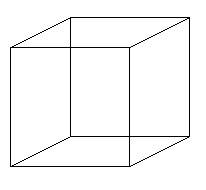
\includegraphics[scale=.7]{images/Necker_cube.png}
      \caption{Necker Cube: Binocular rivalry is due to insufficient sensory information to reach fixation on one explanatory model over another}
        \label{fig:neckerCube}
   \end{center}
\end{figure}


Thus, not only does PC appear to be more computationally efficient, it also promises to be more flexible than alternative models of cognition---facilitated by a second-order mechanism of precision-weighting.  The process of prediction error minimisation accords neatly with the mandate of free energy minimisation prescribed by the AIF.  As I explain in more detail below, the PC paradigm offers an opportunity to efficiently and flexibly integrate various sensory inputs (exteroceptive, interoceptive, and proprioceptive) into one overarching cognitive process.


\myparagraph{Was it a thief or just the wind?\label{sect:windThief}}
To understand how the PC account applies to human cognition, consider the following example used by cognitive scientist Giovanni Pezzulo \textcite{Pezzulo2013}.  Imagine you wake up in the middle of the night to the sound of your bedroom window creaking.  At the higher levels of the predictive coding architecture, competing perceptual hypotheses emerge to explain the likely causes of the sensory experience.  For simplicity, assume that two plausible hypotheses emerge: 1) the wind outside caused the window to creak (wind), or 2) a thief is trying to break in to your house (thief).  The probability that the sensory experience of the window creaking is due to the wind can be represented by the equation in Figure ~\ref{fig:windThief}.  The predictive coding proposal is that the brain formulates a probability estimate based on:

\begin{enumerate}
  \item $P(wind)$: the model \textit{prior} formulated by previous experience (e.g., it has been windy at night recently, or in the case of $P(thief)$, there have been some recent thefts in the neighbourhood)
  \item $P(evidence|wind)$: the \textit{likelihood} that the sensory experience is caused by the wind (this value could be informed by other sources of information, e.g., the trees outside are also rustling, the dog is not barking (which may be the case if it were a thief, ($P(evidence|thief)$))
  \item Precision weighting: the reliability or certainty associated with your sensory inputs (it is dark in your room and so you may not trust your visual perception, you just woke up so could have been dreaming, etc.).  The precision weight is factored into the ``evidence.''
\end{enumerate}


\begin{figure}[htbp]
  \begin{center}
    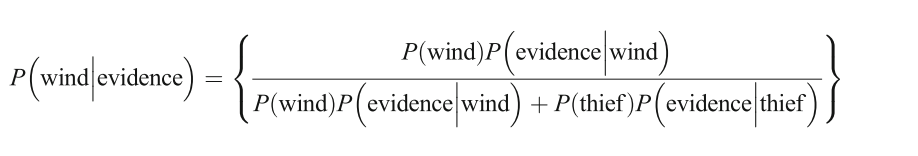
\includegraphics[scale=.5]{images/windThief.png}
      \caption{Bayesian model for the prediction of wind as the cause of the window creaking. Source: Pezzulo (2014)}
        \label{fig:windThief}
   \end{center}
\end{figure}

These two hypotheses (wind and thief) effectively compete on the basis of how well they explain the sensory stimuli.  The brain's capacity to quantify the uncertainty of any given sensory state (precision) facilitates optimal selection between competing predictions pertaining to the same bottom-up sensory signals.  In the wind vs. thief example, based on the the priors ($P(wind) = .8$ (it has been windy recently) and $P(thief) = .2$ (no recent reports of theft)), and the (precision-weighted) evidence ($P(evidence|wind) = .6$ and $P(evidence|wind) = .5$ (roughly equivalent because it is dark and you have just woken up), the probability of wind ($= .8276$) is much higher than the probability of thief ($= .1724$).  In this case, the prediction that wind caused the window to creak wins out, and guides action and perception accordingly (you decide to go back to sleep).


\myparagraph{Why is active inference ``active?''}
Original models of PC dealt primarily with ``exteroceptive'' information \citep[relating to stimuli that are external to an organism, i.e. visual, auditory, haptic perception][]{Rao1999,Friston2010}.  In the wind vs. thief model considered above, only exteroceptive evidence is considered, in the form of the auditory stimulus of the window creaking.  Research has since demonstrated that the PC approach can also account for ``proprioceptive'' information (relating to stimuli that are produced and perceived within an organism, especially those connected with the position and movement of the body), as well as ``interoceptive'' information  \citep[relating to stimuli produced within an organism, particularly by the body's organs (viscera) e.g., ``gut feelings,'' or elevated heart rate; see][]{Seth2013,FeldmanBarrett2015}.  Incorporating proprioceptive and interoceptive information sources into PC allows researchers to theoretically demonstrate that human cognition is both ``embodied'' \citep[inference is rooted in and contingent upon visceral, interoceptive information][]{Pezzulo2014}, as well as ``active'' \citep[in the sense that humans can move throughout the environment to reduce the discrepancy between proprioceptive predictions and actual body states, see][]{Friston2010,Clark2015}.

In the case of motor systems, agents are able to move their sensors in ways that amount to actively seeking or generating the sensory consequences that they (or rather, their predictive models) expect.  In this way, ``error signals self-suppress, not through neuronally mediated effects, but by eliciting movements that change bottom-up proprioceptive and sensory input'' \citep[][1349]{Friston2003}.  The hierarchical and nonlinear structure of predictive coding enables diverse sensory inputs feed into the same inferential mechanism.  Diverse functions of action, cognition and perception are thus integrated into an framework that is both embodied and enactive \citep{Friston2015}.  Embodied and active sources of information broaden the scope of human cognition beyond the brain and reduce reliance upon computationally intensive mental simulation as a driving force for action.  Instead, canny utilisation of extra-neural and bio-external affordances of the environment can support free energy minimisation \citep{Clark2015}.  Thus, the \textit{integrative} approach of the AIF allows for a conception of interlocking traditionally disparate sources of information---e.g., physical, emotional, and cognitive---into one inferential process.

Consider an embodied and active revision of the wind vs. thief example.  Two key differences in the model become apparent.  First, the evidence considered is broadened to include both interoceptive and proprioceptive information, in addition to exteroceptive evidence.  Assume that before you went to bed you just watched a horror movie, and when you woke up to the sound of a window creaking your heart began to pound and you immediately fixated on the hypothesis that a thief was causing your window to creak.  Fixation on the thief hypothesis can be explained by the contribution of interoceptive information (e.g., autonomic stress response, heart beat, etc.) to sensory the evidence \citep{Pezzulo2014}.  In addition, the incorporation of proprioceptive information into the model (for example, the possibility of moving to turn on the bed-side lamp) creates additional cognitive affordances through which higher level predictions could be strengthened (or free energy can be minimised).  This difference in the model demonstrates how perception, emotion, and action are functionally integrated in human cognition.

Second, broadening sensory inputs in the model also introduces the problem of differential reliability of sensory inputs.  The wind vs. thief example describes a situation in which exteroceptive information is relatively unreliable: it is dark so visual inputs are restricted, and what you heard is unreliable because you just woke up and maybe it was part of a dream.  By contrast, interoceptive information is usually quite certain: you can be certain that your heart is pounding and that you feel unnerved.  In this particular case, interoceptive inputs may have a greater influence on the overall inference.  As explained above, evidence suggests that the brain deals with multiple sensory inputs via a process of ``Bayesian multisensory integration'' \citep{Ernst2004}, with the reliability of each sensory input proportional to the inverse of its variance.  In the wind vs. thief example, the interoceptive information from your body, precision-weighted as the most reliable source, will likely tip the model to favour the hypothesis that it is a thief, in which case you will move your body in ways that reconcile discrepancy between proprioceptive predictions that also correspond to the thief hypothesis, and therefore are tuned to a higher volume in the model. The result of this trajectory of action and perception may be that you act to on on your bedside lamp \citep{Pezzulo2014}.

Thus, the combination of mutlisensory integration (of exteroceptive, proprioceptive, and interoceptive information) and Bayesian precision-weighting of prediction errors provides the necessary mechanics for a conception of human cognition that is both active and embodied.    In the following section, I introduce the concept of affordances as a necessary compliment to the PC paradigm and a core component of the AIF.

%Even if turning on the light would subsequently reveal that it was the wind all along,

%[; for a detailed discussion of the differences between traditional and active inference approaches to motor control, see Appendix ~\ref{app2:theory} Section  ~\ref{app2:motorControl}]  In the next section, I explain how active inference can be applied to joint action and shed light on the phenomenon of team click.



\subsubsection{Affordances}
In this section I introduce the concept of affordances and its relevance to the AIF.  In brief, affordances can be understood within the AIF as extra-neural resources that couple with generative models to produce loops of action and perception \citep{Ramstead2016,Clark2015}.  The concept of affordance is crucial to facilitate an understanding how active inference unfolds in real-world settings.  While affordances have traditionally been studied narrowly as localised resources for basic perception, researchers working with the AIF have proposed an extension of the the concept of affordances to include a spectrum of objects, ranging from content-limited ``natural affordances,'' through to content-rich affordances mediated by cultural conventions and institutions \citep[cf.][]{Roepstorff2010,Ramstead2016}.

The theory of affordances, originally proposed by psychologist \textcite{Gibson1979} states that the world is perceived not only in terms of object shapes and spatial relationships, but also in terms of object possibilities for action.  This definition accords neatly with the propositions of the AIF, which posits Bayesian inference machines reliant on cognitive resources distributed throughout brains, bodies, and physical features of the task-specific environment in circular causal loops of perception and action.  Put simply, an affordance is the attribute of a hidden cause in the environment that induces (through PC architecture) predictions \citep[908]{Pezzulo2013}.  Repeated coupling between generative models and their extra-neural correlations in the environment give rise to dense causal relations between particular affordances and particular predictions.

Working within the AIF, \textcite[7]{Ramstead2016} propose that the extra-neural cognitive resources to which generative models couple (i.e., affordances) can be understood as a spectrum, with ``natural affordances'' at one end, and ``conventional affordances'' at the other \citep{Ramstead2016}.  Natural affordances pertain mainly to basic correlations between the organism and the environment that enable sensorimotor control and regulation: the physical features of the environment; the ground beneath our feet.  Conventional affordances, by contrast, often rely on consensus from other agents and culturally derived regularities; the carpet beneath our feet, or the keys at our fingertips, for example.  As Ramstead and colleagues explain:

\begin{quote}
  Successfully learned human conventions that govern action are also best conceptualised as affordances. Such affordances depend on shared sets of expectations, reflected in the ability to engage immersively in patterned cultural practices, which reference, depend on, or enact folk ontologies, moralities and epistemologies. We might call these ``conventional'' affordances.
\end{quote}

As \textcite[906]{Pezzulo2014} points out, PC hierarchies extend well beyond hypotheses concerning the source and reliability of immediate sensory inputs. At higher levels of the PC hierarchy, more profound regularities can be represented, such as long-term beliefs that are increasingly more removed from sensorimotor events. In humans, while higher order beliefs may be acquired mainly through cultural learning (rather than purely ``from the ground up'' via natural affordances),  these beliefs may still remain ``grounded'' through the linkage with lower-level sensory events).  Indeed, higher-order beliefs may need to remain grounded in sensory experience in order to retain long-term viability.

\textcite{Bruineberg2014} propose that affordances should be conceived of using a three-step topology. For any given agent, there exists a ``landscape'' of all possible affordances, within which an agent only engages with a specific ``field'' of affordances prescribed by the patterned coupling between predictive models and natural and cultural features of the environment; the affordances to which an individual brain is coupled at any one moment can be understood as ``solicitations.''  This three-level topology of affordances allows for a conception of the way in which repeated agent-environment coupling can give rise to particular regimes of attention, action, and perception within a vast landscape of all possible affordances.

When a specific field affordances or set of solicitations are conventional and shared, repeated coupling can generate regimes of \textit{shared} attention. For the purposes of this dissertation, conventional (cultural) affordances can thus be understood as regularities in the environment that cue multi-modal predictions for joint action.  This understanding incorporates factors that are traditionally understood to b psychologically explicit or ``external,'' such as societal values or similar cultural dimensions, \citep{Hofstede1991,Schwartz1992}, social practices and artefacts  \citep{Nisbett2003a}, as well as and ``internal,'' such as dominant modes of self-construal or dispositional and linguistic tendencies \citep{Markus1991}.  The concept of affordances enables an extension of the AIF beyond immediate sensorimotor processes, and into the domain traditionally understood as ``culture'' \citep{Roepstorff2010}.

In sum, the concept of affordances is an indispensable compliment to generative models of the AIF.  As discussed in the previous section (Section ~\ref{sect:predictiveCoding}, generative models can be understood as containing a spectrum of statistical complexity, ranging from basic (content-free) to elaborate (and seemingly content-rich) correlations.  The affordances to which these models couple (and therefore on which such models depend) can likewise be conceived of as existing on a spectrum, spanning natural and conventional (cultural) variants.  Importantly, the concept of affordances reveals the fact that higher-order generative models are contingent on couplings with higher-order affordances, i.e., culturally shared affordances.  In other words, higher cognitive processes are fundamentally social processes.   The correlation in complexity between generative models and their affordances provides a proximate explanatory mechanism for the observable fact that higher-order cognitive capacities for belief, reason, and language appear to be fundamentally contingent social and cultural processes, rather than purely innate capacities for which humans are naturally endowed \citep{Sperber1997,Henrich2015}.  The concept of affordances also offers an explanation for observable cross-cultural variation in action, perception, and attention \citep[cf.][]{Nisbett2003}.  Selective engagement with specific fields of affordances give rise to regimes of shared attention and beliefs that direct trajectories for individual and collective activity.


\myparagraph{Summary of the active inference approach to joint action}
To summarise, the AIF entails a radical inverse of traditional models of cognition that rely predominantly on bottom-up sensory inputs and top-down feature detection \citep[e.g.,][]{Marr1985}. Instead, active inference posits that top-down predictive models themselves shape perception and action, and the only information that travels forward (or from the ``bottom-up'') is the error signals that arise from discrepancies between predictions and the sensorium \citep{Pickering2014}.  AIF depicts a human cognitive system in which perception, mental simulation, emotion, and action are functionally and temporally integrated to manage uncertainty (free energy) inherent in interactions with the environment \citep{Clark2013}.  Importantly, these processes of generative modelling are dynamically coupled with affordances that span a spectrum of basal natural correlations with the physical features of the environment, through to elaborate culturally mediated beliefs and conventions.  The integrative approach of AIF allows for a theorisation of the interlocking physical, affective, and social dimensions of group exercise.


\section{Active inference applied to joint action \label{sect:activeInfJA}}
As explained above, traditional theoretical models of human cognition have struggled to integrate cognition with emotion, mental simulation with habitual response, flexibility with efficiency \citep{Clark2015}.
Team click is a powerful subjective experience in which many of these binaries appear to collapse and co-occur.  The AIF approach promises a testable theory of the embodied and dynamic dimensions of joint action.  In this section, I outline existing attempts to apply the AIF to joint action, and point to predictions relevant to team click and social bonding in joint action.
%, which appear to be maximised in team click.

%\myparagraph{Auxiliary approaches to joint action}
The AIF proposal offers a more integrative alternative to existing models of joint action, which rely on mechanisms of sensory prediction (of self, other, and joint actions) that are individually-bounded and auxiliary to joint action itself \citep{Pesquita2017}.   \textcite{Keller2016}, for example, presented a conceptual framework that applies an ``auxiliary forward model'' (AFM) approach to musical joint actions.  The AFM approach requires that agents produce predictive models responsible for individual action planning and control (self-internal models), prediction of others' actions (other-internal models), and representation of the shared goal (joint-internal models).  Of these three types of models, however, only self-internal models comprise the auxiliary predictive architecture (i.e., the forward model containing an efference copy of one's own action, and ``inverse models'' that are responsible for output of motor commands ~\ref{app2:theory}, Section ~\ref{app2:motorControl} for a more detailed explanation of these terms).  Thus, both anticipation and compensation in joint action depends on a control loop, whereby sensory information (error signals) are routed (fed-back) through self-internal models, which inform the production of auxiliary predictions---of self, other, and joint action---grounded in individual motor simulations.  Importantly, in this model,  error signals are fed-back only to the self-inverse model, as no inverse model for the joint action partner exists.

The longstanding proposal that individuals only produce auxiliary predictive models of their own actions (as opposed to others' actions too) has served to explain how individuals effectively attend to others in joint action.  With privileged access to an efferent copy of impending individual action, an agent is able to preemptively attenuate sensitivity to their own action, in order to attend to the actions (and prediction errors) of others \citep{Wolpert1998}.  For example, the AFM approach provides an explanation for the phenomenon of tickling, or specifically why it is near impossible to tickle oneself \citep[due to sensory attenuation resulting from the self-generated predictions about the consequences of action][]{Blakemore2003}. However, while the AFM has proven adequate to explain individual motor control, and some instances of joint action (such as tickling), it also contains potential shortcomings when applied to dynamical joint action scenarios.

\textcite{Pesquita2017} summarise three shortcomings when applying AFM to joint action.  First, the AFM model assumes a static and unchanging representation of the shared goal and the other's goal, and provides no mechanism through which the shared goal representation can be dynamically updated (based on prediction error signals).  This issue limits the ability of AFM to account for the real-world flexibility and interchangeability of shared goals (for example, the adaptive switching between the shared goal of carrying a table or the bench depending on the location of both objects).  Second, the same rigidity applies to other-inverse models.  The inability to directly and dynamically update other-models suggests the practical possibility that self and other models may gradually diverge over time due to the lack of sufficient predictive information regarding the actions of others \citep{Pickering2014}. Third, the AFM approach does not specify how sensory input is differentially used to update self and other models, which limits the model's ability to account for learning and adaptation within joint action \citep{Pesquita2017}.  Thus, not only does the AFM approach appear to be computationally intensive (due to the recruitment of auxiliary inverse models and dual motor commands, discussed in Section ~\ref{sect:predictiveCoding}), it also appears to be unable to fully account for the dynamic flexibility of real-world joint action.

\myparagraph{Generalised synchronisation as a foundation for joint action}
The AIF offers a thoroughly dynamical approach to joint action, whereby two (or more) Bayesian predictive brains committed to modelling each other in order to minimise free energy \citep{Friston2015,Friston2015a}. In order to achieve free energy minimisation, the sensory stimuli produced by co-actors in joint action must be pre-emptively modelled, just like other features of the sensorium (as explained above, see Section ~\ref{sect:thermoCog}).  This necessitates a scenario in which brain A has a model of brain B, which includes the fact brain B is modelling brain A, and so on---\textit{ad infinitum}.

The recurrent predictions of both brains about one another threatens an infinite runaway regress that could preclude accurate modelling of either brain.  However, as Friston and Frith demonstrate formally (mathematically), this recursion dissolves if the models of the two brains are formally similar \citep{Friston2015}.  When grounded in computational similarity, each brain is able to generate predictions of the sensory outcomes caused by itself and the other in the same way.  The authors propose that this will lead to dynamical ``generalised synchronisation'' \citep{Barreto2003}, or dynamical coupling between the internal models of both brains (for a more detailed explanation of general synchronisation and its dynamical underpinnings, see Appendix ~\ref{app2:theory} Section ~\ref{sect:generalSync}).  In this way, two or more brains are able to accurately predict each other's behaviour based on feedback of exteroceptive (sensory information from the actions of others and the task environment) and proprioceptive (pertaining one's own contribution to joint action) prediction errors.  In essence, other agents exist as affordances to which individual brains couple, and upon which individual brains become dependent for ongoing (joint) processes of action, perception, and attention.

In place of auxiliary processes of prediction, the AIF for joint action hinges instead on the function of precision weighting of prediction errors in order to facilitate and finesse joint action.  When performing action, the individual turns down the volume (reduce the precision weighting) on prediction errors relating to one's own action so that movement can occur unimpeded by over-attention to self-generated prediction errors \citep[an intuitive example of the opposite of this ideal scenario is when the flow of speech is interrupted due to the availability of exteroceptive auditory feedback in the case of a Skype call][]{Friston2015}.  Alternatively, when attending the the action of others, the attenuation of proprioceptive error signals can cease. In this way, precision weighting is used to flexibly adjust the volume of multi-modal prediction errors (exteroceptive, interoceptive, and proprioceptive) in order to finesse and sustain generalised synchronisation (the shared narrative on which joint action is sustained).

Heuristically, this suggests that active inference in joint action takes one of two modes; either 1) flexibly attending to sensations or
2) acting during periods of sensory attenuation \citep{Friston2015}.  The active inference explanation for ticklishness, for example, is an inferential mode in which the volume on proprioceptive prediction error is ``dialled-up.''  The failure of self-tickling, by contrast, pertains to a mode of active inference in which the volume of proprioceptive prediction is ``dialled-down'' to enable smooth flow of action execution.
  \footnote{Recall also that instances of tickling commonly involve a stationary victim. While it indeed appears almost impossible to tickle oneself, it is also rare to be tickled while moving, i.e., acting during periods of sensory attenuation.}


\myparagraph{Predictive Joint Action Model (PJAM)\label{sect:PJAM}}
\textcite{Pesquita2017} have formulated a minimal architecture for an active inference approach to joint action, which they term a ``Predictive Joint Action Model'' (PJAM).  PJAM is comprised of three hierarchical levels of inference: goal representation, action-planning, and sensory routing (see figure ~\ref{fig:PJAM}).  Each level of the hierarchical model is informed by prediction errors from the level below, and the model works iteratively to minimise free energy in joint action scenarios.  In line with the AIF, PJAM does away with auxiliary processes of motor control and efferent copies, and posits instead that joint action emerges directly from two or more individuals reaching generalised synchronisation by converging on equivalent predictive models for joint action \citep{Friston2015}.

  \begin{figure}[htbp]
    \begin{center}
      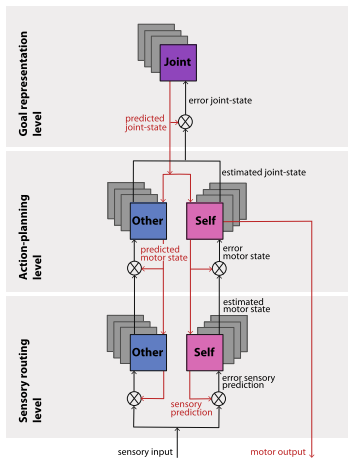
\includegraphics[scale=.8]{images/PJAM.png}
        \caption{The Predictive Joint Action Model \citep{Pesquita2017}}
          \label{fig:PJAM}
     \end{center}
  \end{figure}

In contrast to the AFM approach, which posits a shared goal representation deriving from self-internal models, the PJAM suggests that a shared goal derives primarily from the dynamical coupling of agents to each other and to other (shared) affordances of the task-specific environment.  Thus, rather than being wholly explicit, propositional, or pre-set, the shared goal is understood to span the entire predictive hierarchy, with basal coupling of sensorimotor processes at the lower end, through to more elaborate models that facilitate more explicit or propositional content, at the higher end.  In a bidirectional cascade of prediction and prediction error, the ``shared narrative'' at the goal representation level generates discrete action plans for self and other, which are then tested against prediction errors arising from the sensory routing models below \citep{Pesquita2017}.


\subsubsection{Evidence in support of PJAM}

PJAM (and the AIF which it extends) predicts that joint action will be established and maintained through generalised synchronisation between two or more predictive brains driven by an overarching mandate of free energy minimisation \citep{Friston2015}.  In particular, PJAM predicts that co-actors in joint action will generate predictive models that reflect 1) a shared goal, 2) action plans for self and other, and 3) routing instructions for sensory inputs.  Consistent with the modelling view of the AIF (see Section ~\ref{sect:thermoCog}), these three layers of generative models will reflect an hierarchy of complexity, and will be coupled to a continuum of natural and conventional affordances.  Below I outline existing experimental evidence in support of these predictions.


\myparagraph{Evidence for generalised synchronisation in joint action}
Evidence that musicians maintain shared representation of desired unified sound of an ensemble \citep{Keller2008}, track deviations from desired joint state \citep{Loehr2013}, and allow shared goal predictions to guide future action \citep{Loehr2016}, confirms the hypothesis that co-actors share a dynamical and flexible shared goal---a shared narrative or common ground.  PJAM specifically predicts that the foundation for this shared narrative will be dynamical, i.e., it will involve coupling of system component degrees of freedom of co-actors in joint action \citep{Turvey1978,Schmidt1990}. Dynamic coupling can be identified by two core properties:  1) dimensional compression (potentially independent DF are coupled so that the synergy possesses a lower dimensionality than the set of components from which it arises) and 2) reciprocal compensation \citep[the ability of one component of a synergy to react to changes in others][]{Riley2011}.

An accumulation of evidence on multiple levels of human behaviour, from brain function \citep{Yufik1998,Sengupta2013}, to interpersonal interactions \citep{Kelso2009,Riley2011,Fusaroli2014}, to large-scale human societal dynamics \citep{Nowak2017} supports the existence of dynamic coupling.  In the case of joint action in particular, individuals have been found to couple and reciprocally constrain their movements reducing the overall control needed to maintain effective cooperation \citep{Ramenzoni2011,Ramenzoni2012,Riley2011,Schmidt1990}.  Studies of real-world joint action scenarios such as dancing, martial arts, and moving objects like furniture have revealed evidence for dynamic coupling between co-actors.  In these studies, specific component degrees of freedom are modelled as coupled oscillators \citep[using the HKB model, which describes the change in the relative phase between two oscillatory components. See][]{Haken1985,Kelso1986}.  Interestingly, dynamic coupling of movement has been measured beyond dyadic synchronisation, in the analysis of sub-phases of team sports \citep{Passos2014,Duarte2012} and group dancing \citep{Chauvigne2017}.  For a more thorough explanation of dynamic coupling in human movement systems, including methods for measuring dynamical quantities, see Appendix ~\ref{app2:theory} Section ~\ref{app2:dynamicCoupling}.

This evidence is supported by recent research focussed on the movement signatures of joint action that resemble instances of ``identical synchronisation,'' or the idea of being ``in the zone'' with a co-actor. Working within the common dyadic ``mirror game'' paradigm, \textcite{Noy2011,Noy2015,Hart2014} have identified ``co-confident motion'' (CC motion) as a canonical movement pattern of synchronised motion characterised by smooth and jitter-less motion, without the typical jitter resulting from reactive control in more commonly encountered leader-follower patterns.  In CC motion, different players appear to shift their basic motion signatures to a movement shape that is altogether different from their individually preferred shapes \citep{Hart2014}. Importantly, the pattern of CC motion shares the same sine wave shape as the optimal solution of the minimum jerk model, a well-known motor control model for rhythmic motion \citep{Hogan2007}.  This evidence accords with the proposal that joint action is underwritten by a ``shared narrative'' that transcends individual action tendencies of self and other and produces a  ``we-mode'' of social cognition (exemplified by CC motion) \citep{Gallotti2013}.

\myparagraph{Evidence for self and other action plans}
On the level of self and other action plans, experimental evidence suggests that co-actors generate internal models of self and other either spontaneously and involuntarily---as in the commonly used social simon task experimental paradigm \citep{Sebanz2003,Atmaca2008}---or more deliberately---as in a coordinated dyadic horizontal jumping task \citep{Vesper2012}.  \textcite{Loehr2016} demonstrate that when learning a joint piano piece, musicians are able to better perform a piece together rather than solo, which suggests that representations about each participant in joint action are encoded within the joint context of the interaction.  Studies also show that the capacity for co-representation of self and other action plans is modulated by mood \citep[positive or negative affect, see][]{Kuhbandner2010}, self-concept and social orientation \citep{Colzato2012,Colzato2012a}, and processes of group membership \citep{DeBruijn2008,Iani2013}. This evidence lends support to the proposal that active inference involves coupling with various natural and conventional affordances in order to flexibly integrate information deriving form various sensory inputs.

The evidence outline immediately above is supported by parallel strands of research in psychology \citep{Prinz1990,Prinz1997,Prinz2013}, neurophysiology \citep{Rizzolatti2004,Rizzolatti2010}, and neurocognition \citep{Wolpert1998,Wolpert2000} that interpersonal behavioural coordination in joint action is facilitated by the intrinsic links between action perception and action execution in the human brain.  In essence, action-perception coupling refers to the ostensive co-occurrence of a stimulus for action and its motor representation.  For example, for individuals who have mastered a certain sensorimotor task, the representation of a perceptual effect (say the sound of a middle-C on a piano) can trigger the movement necessary to produce the effect itself (motor instructions for playing the middle-C key on a piano) \citep{Novembre2014}. Evidence suggests that skilled individuals not only develop generative models for self action, but also for the actions of others in joint action \citep{Novembre2012}. Action-perception links can be used for monitoring and integrating (e.g., timing or combined pitches) the actions of other ensemble members with self-generated actions \citep{Loehr2013}, and these effects appear to be stronger in individuals with high perspective taking skills \citep{Novembre2012,Loehr2013}.  The overlap between mechanisms for action production and action observation suggests that individuals may represent their own and others’ actions in a commensurable format.  Training-induced motoric representation of self and other actions may facilitate various capacities important for joint action, such as prediction, adaptation, and entrainment (for a more detailed treatment of action-perception links and their relevance to joint action, see Appendix ~\ref{app2:theory} Section ~\ref{app2:actionPerceptionLinks}).

\myparagraph{Evidence for sensory routing}
On a sensory-routing level, evidence suggests that modulation in sensory attenuation is driven by the predictability of the outcome, as opposed to necessarily being driven by the presence or absence of auxilliary efference copies \citep{Sato2008}.  In addition, attributing sensory consequences to joint action partners is linked to cooperative success \citep{Chaminade2012}, suggesting that finely tuned sensory routing based on predictions of self and other actions could be key to successful coordination.



\subsubsection{Summary of PJAM and implications of AIF for team click and social bonding}

In sum, PJAM provides a framework for the function of active inference in processes of alignment and movement coordination in joint action.  Each level of PJAM generates predictions of the information that it expects to be found on the level below.  The radical proposal of the AIF for joint action is that, unlike the AFM approach, the AIF formally theorises the way in which cognitive resources are shared between two or more brains, bodies, and the task-specific environment \citep{Clark2015}.  Therefore, social connection in joint action can be conceived as dynamic coupling between agents, which spans a continuum of basal sensorimotor processes, through to higher order beliefs facilitated by regimes of shared attention.  In this sense, social connection in joint action could arise in situations in which individuals perceive click between co-actors and other affordances contained within a certain field of activity.  In this dissertation, I develop the idea that in real world joint action scenarios such as interaction team sport, co-actors interact and rehearse their behaviours to produce a hierarchy of aligned representations, an implicit ``common ground'' \citep[cf.][]{Noy2017} on which joint action can unfold, and social connection may be found through team click.

%we are already connected!! (China, fusion)
%This ``shared narrative'' which supposedly transcends agency, is supported by the self-organising



\section{Active inference in group exercise \label{sect:activeInfGE}}

In the previous section I reviewed evidence in support the AIF for joint action.  The AIF begins with the assumption that, on a basal level, joint action consists of two or more Bayesian inferential systems attempting to minimise free energy by modelling the hidden causes of sensory stimuli.  From sheer computational perspective, joint action is an inherently challenging task, but it appears that ``general synchronisation'' derived from the coupling of two or more agents facilitates a shared narrative (functionally equivalent models for joint action).  This perceptual common ground resembles a situation in which ``adjustments for ``Am I?'' and ``Are You?'' and ``Where Are We?'' and stuff like that...'' (see Section ~\ref{sect:teamClickIntro}) dissolve, and a transcendent ``we-mode'' of collective agency is glimpsed \citep[][]{Friston2015}.  Anecdote and observation of real-world joint action scenarios suggests that achieving the ``click'' of joint action---in spite of its uncertainty, and however momentarily it lasts---can be a deeply rewarding experience.  In the case of joint action in group exercise contexts, it appears that various features of group exercise serve to amplify both the challenges of joint action, and the psycho-social costs and rewards possible through adherence.

\myparagraph{Group exercise involves multi-agent (and not just dyadic) joint action}
Above and beyond normal day-to-day instances of communication and exchange, joint action in group exercise contexts such as sport place extreme cognitive load on participants. The active inference approach to joint action outlined above is based on preliminary models of dyadic joint action involving turn taking \citep[i.e., in bird song exchanges][]{Friston2015}.  Group exercise contexts, particularly modern sport contexts, often involve large numbers of co-participants, in either ``inter-active'' or ``co-active'' modes of coordination.
    \footnote{
    In co-active sports (e.g., bowling, archery), team members perform separately and the team outcome is a product of combined individual performances. In interactive sports (e.g., volleyball, soccer, rugby), goal accomplishment requires the establishment of complex patterns of interaction and coordination among team members \citep{Filho2014}.
    }
Thus, achieving cognitive synchronisation in joint action of group exercise contexts may be much more difficult.  Evolutionary Anthropologist Robin Dunbar \textcite{Dunbar1992} proposes that the ratio of human neocortex size to total brain volume imposes an upper cognitive limit on real-time coordination of behaviour of approximately four to five individuals.  The sheer computational burden of modelling multiple agents in group exercise may place an unmanageable cognitive load on our normal healthy processes of active inference.  Indeed, at the very least, multi-agent joint action poses a challenge for the existing theoretical model for joint action (PJAM), which is formulated primarily based on dyadic interactions \citep{Pesquita2017}.

\myparagraph{Joint action in group exercise is ``on-line'' and ``in-the-moment''}
Particularly in the case of interactive team sports, interpersonal movement coordination is often executed ``on-line'' and ``in the moment,'' as opposed to step-by-step turn taking.  This fact poses a challenge to Friston and Frith's proposal that active inference in joint action comprises two modes (either actively attending to sensory stimuli, or else moving while in a state of sensory attenuation, see Section ~\ref{sect:activeInfJA} above).  Exactly what occurs when actors need to concurrently move and sense others moving at the same is poorly understood.  What happens to the precision weightings---the volume gauges---on proprioceptive, interoceptive, and exteroceptive prediction errors In instances of dynamic interactive joint action involving co-occurence of movement between agents in joint action?   What is the impact of on-line and in the moment join action on the experiences of agency in group exercise?  Empirical research is yet to provide answers to these questions.

\myparagraph{Group exercise involves competition}
As if the cognitive load of multiple agents and on-line coordination of complex schemas for joint action was not enough for the humble human brain, interactional team sports also usually involves \textit{competition}.  While competition in sport is usually adorned with elaborate social meanings surrounding the ethics of winning and losing \citep{McNamee2008}, on a cognitive level, competition in joint action entails one individual or team of individuals actively attempting to foil or disrupt the predictive models of another individual or team of individuals \citep{Reimer2006}.  The competitive dimension of interactional team sports thus serves to further spike cognitive uncertainty between co-actors in joint action.  The uncertainty involved in competitive joint action scenarios could have further implications for the ability of second-order Bayesian inference concerning the reliability of sensory inputs \citep{Pezzulo2014}.

\myparagraph{Group exercise involves metabolic tradeoffs in the brain}
In addition to these heightened cognitive challenges associated with complex and dynamic joint action in group exercise, high levels of physiological exertion characteristic of group exercise could also serve to spike uncertainty.  Neuroscientist Arne Dietrich draws attention to the fact that physical exercise is at its core a stressor that places extreme energy demands the organism \citep{Dietrich2011}.
Such a situation will necessitate an energy tradeoff in the brain, whereby energetically costly brain regions inessential to movement execution are temporarily downregulated \citep{Dietrich2004b}.  Dietrich suggests that experiences of flow and the ``runner's high'' in exercise could be the result of temporary downregulation of energetically costly brain regions inessential to movement execution  \citep{Dietrich2004b}.  Dietrich and colleagues propose candidate areas of the dorsolateral prefrontal cortex responsible for self-monitoring and proprioceptive sensory attenuation \citep[commonly known as the ``inner critic'' regions of the brain, see][]{Limb2008}.  It is currently not well understood precisely whether or how neurometabolic tradeoffs in the brain could impact upon joint action and the experience of team click.  However, it is conceivable that metabolic tradeoffs in the brain owing to prolonged physiological stress may have implications for the second-order inferential processes of precision weighting sensory inputs.


\subsection{Free energy minimisation in group exercise demands greater reliance on extra-neural affordances \label{sect:extraNeural}}
To summarise, the combination of cognitive demands associated with tracking and modelling multiple agents ``in-the-moment,'' the neurometabolic tradeoffs associated with (often extreme) levels of physiological exertion, and even the competitive dimension of some group exercise contexts (for example interactive team sports), could create an environment in which humans' usual cognitive capacities are strained and compromised.  The fact that experiences of team click are particularly prevalent in group exercise contexts (compared to more mundane or quotidian instances of joint action) suggests that amplification of uncertainty and stress in group exercise could be a critical factor in facilitating powerful psychosocial effects.

The active inference approach would predict that individuals, when faced with the extreme cognitive uncertainty of joint action in group exercise, will tend to preference mechanisms that maximise uncertainty reduction (minimise uncertainty).  In the case of joint action in group exercise, this may entail reliance on predictive models that outsource the computational cost to affordances beyond the brain, or at least the metabolically expensive cortical areas of the brain \citep{Dietrich2004,Clark2015}.  In the case of highly skilled practitioners, whose predictive models for action have been finely tuned to the affordances of the task environment (inlcuding co-actors), it is plausible that extra-neural and even extra-personal resources (e.g., physical features of the task environment) could provide a more cognitively efficient and effective route to the performance of successful joint action and thus the minimisation of free energy.

Various strands of evidence support these predictions.  Studies of highly skilled practitioners in joint action demonstrate that more technically competent practitioners generate more accurate predictive models for joint action than less technically competent practitioners \citep{Tomeo2012,Aglioti2008,Mulligan2016}.   In studies involving skilled versus non-skilled practitioners in dyadic interactions, it has been shown that more skilled practitioners create stronger dynamical coupling through flexibly modulating their actions with others \citep{Schmidt2011,Caron2017}. These findings are corroborated by other studies that find that professional footballers (versus novice controls) are able to more accurately predict the direction of a kick from another player's body kinematics (\cite{Tomeo2012}, see also \cite{Aglioti2008,Mulligan2016} for similar results with basketball and dart players).  When analysing co-regulation between members of basketball teams, \textcite{Bourbousson2015} showed that more expert teams made fewer mutual adjustments (at the level of the activity that was meaningful for co-actors), suggesting an enhanced capability of expert social systems to achieve and maintain an optimal level of awareness during the unfolding activity.

A recent field study with expert rowers revealed that athletes predominantly utilised
extra-personal (rather than inter-personal) regulation processes in order to facilitate and sustain joint action, and attention to interpersonal regulation occurred only during instances of expectation violation concerning performance in joint action \citep[; for a full explanation of this study, see Appendix ~\ref{app2:theory} Section ~\ref{sect:rowerStudy}]{RKiouak2016}. These results suggest that athletes used the affordances of the environment to mediate the arrangement of individual and joint activities \citep{Bourbousson2011,Bourbousson2012}.  Taken together, this evidence supports the prediction for a tendency for co-actors in joint action to utilise neurocomputationally conservative models and coupling with extra-neural affordances under circumstances of high levels of free energy (such as those common to group exercise).


\subsection{Team click and the dark room dilemma}
The evidence reviewed above demonstrates the human ability to flexibly deploy a range of cognitive strategies, seemingly towards the ultimate goal of free energy minimisation.  Inherent in the application of the free energy principle to group exercise is the paradox that group exercise is an activity that appears to deliberately amplify uncertainty.  In the active inference proposal outlined above, humans are depicted as free-energy minimising systems, driven by the ultimate goal of reducing surprise and maximising efficiency in their interactions with the environment \citep{Friston2010}.  Why do humans seek out and receive high rewards through activity in environments riddled with uncertainty?

On the face of things, the free energy mandate suggests an ``ultimate stable state'' \citep{Mumford1992}, in which all surprise minimised.  As evocatively described by Mumford:

\begin{quote}
  How can a neural imperative to minimize prediction error by enslaving perception, action, and attention accommodate the obvious fact that animals don’t simply seek a nice dark room and stay in it? Surely staying still inside a darkened room would afford easy and nigh-perfect prediction of our own unfolding neural states? Doesn’t the story thus leave out much that really matters for adaptive success: things like boredom, curiosity, play, exploration, foraging, and the thrill of the hunt? \citep[243]{Mumford1992}
\end{quote}

The simple response is that animals (humans included) live and forage in a changing and challenging world, and hence ``expect'' to deploy quite complex strategies to stay within our species-specific window of viability \citep{Bruineberg2014}.  As Clark explains,

\begin{quote}
  Change, motion, exploration, and search are themselves valuable for organisms living in worlds where resources are unevenly spread and new threats and opportunities continuously arise.  This means that change, motion, exploration, and search themselves become predicted and enacted accordingly \citep[193]{Clark2013}
\end{quote}


Agents infer a policy that minimises surprise by minimising the difference (or relative entropy) between likely and desired outcomes, which involves both pursuing the goal-state that has the highest expected utility (often termed “exploitation”) and visiting a number of different goal-states (“exploration”). Crucially, the opportunity to visit new states increases the value of the current state. Casting decision-making problems within a variational framework, therefore, predicts that our behavior is governed by both the entropy and expected utility of future states. This dissolves any dialectic between minimizing surprise and exploration or novelty seeking.
(Schwartenbeck2013)

There is evidence to suggest that the tradeoff between free energy minimisation and the search for novelty, creativity, and play (i.e., uncertainty) appears to be supported by a regime of affective rewards calibrated to precision-weighting dynamics \citep{Chetverikov2016}.
The details of these proximate mechanisms could shed light on the phenomenon of team click and its associated downstream psychosocial effects, including social bonding and social cohesion.  Joint action in group exercise, and the phenomenon of team click in particular thus offers a fascinating space in which to investigate the social cognition of active inference in joint action.  Active inference provides a theoretical frame through which the social cognition of joint action can be more clearly rendered and comprehended.

%How, then, do we explain the widespread prevalence of group exercise contexts, which appear to be riddled with uncertainty owing to the overwhelming complexity of joint action requirements and extreme physiological demands?  The phenomenon of team click could lie at the heart of an explanation to this paradox.

\section{A novel theory of social bonding through joint action\label{sect:novelTheory}}

As explained above, the explanatory power of PJAM in particular (the AIF more generally) lies in its capacity to incorporate various cognitive strategies within one overarching mandate of free energy minimisation \citep{Clark2015}.  The distinction between cortical and extra-cortical, mental and emotional, model-based and model-free cognitive processes dissolves, and in place of these dualisms, a continuum of cognitive strategies are flexibly deployed to exploit brain, body, and bio-external resources \citep{Pezzulo2013}.  Bayesian optimisation facilitates flexibility: the volume on sensory prediction error signals is either ``dialled-up'' or ``dialled-down,'' depending on their reliability judged by prior experience (inverse of variance of the prior distribution). Thus, just as the binary distinction between mental and emotional collapses, so too does the distinction between external and internal, exteroceptive and interoceptive \citep[and proprioceptive][]{Seth2013}.

This conception of joint action allows for a full consideration of the interlocking physical, cognitive, and social processes outlined in in Chapter ~\ref{chap:intro}.   Anecdotal and observational evidence suggests that team click is at once mental and embodied, cognitive as well as emotional, metaphysical (i.e., mysterious) as well as deeply ``visceral'' (see Chapter ~\ref{chap:intro} Section ~\ref{sect:adrian}).  Evidence discussed above suggests that optimal solutions to joint action confined to scenarios like group exercise may tend to favour the recruitment of more extra-neural resources as a way of minimising free energy, whereas less efficient solutions to joint action may rely on more computationally intensive procedures in order to reduce free energy (see Section ~\ref{sect:extraNeural}).  The social cognition of these processes in joint action have not yet been closely considered \citep[but see ][]{Marsh2009,Lumsden2012}.

The link between interpersonal coordination and social bonding has been addressed in the behavioural mimicry and synchrony literatures \citep[e.g.,][]{Wheatley2012,Launay2016,Mogan2017}, but there is less substantive evidence in relation to dynamic interpersonal coordination in natural joint action settings such as those found in group exercise contexts \citep{Marsh2009,Miles2009,Lumsden2012}.  As discussed above, the AIF for joint action suggests that successful performance in joint action will require a continuum of generative models tightly coupled to a spectrum of natural and conventional affordances \citep{Clark2015}.  The cognitive mechanisms that generate subjective perceptions of multimodal alignment between co-actors---what I term team click---could explain the relationship between joint action and social bonding in group exercise.

In the sections that follow, I propose a novel theory of social bonding through joint action, mediated by the phenomenon of team click. I do so by first explaining how joint action typical of group exercise can generate team click, and second how team click can lead to social bonding.

\subsection{Perceptions of success in joint action predict team click\label{sect:JASuccessTeamClick}}

The components of team click outlined above indicate that this often observed phenomenon contains elements of positive expectation violation or surprise, deriving from an experience of tacit or implicit coordination in joint action.  The phenomenology of team click can also involve the blurring of boundaries between self and others in the team, the perception of ``atmosphere'' or aura surrounding the group, as well as a perception of reliability of teammates and the self to successfully perform joint action.

How does joint action in group exercise generate the experience of team click?  Considered from an active inference perspective, joint action in group exercise creates a unique environment for processes related to social cognition. In short, group exercise contexts involve high levels of cognitive uncertainty.  Group exercise involves high cognitive load associated with complex joint action requirements involving many actors, many hierarchical layers of joint goals over various sensory modalities and spatiotemporal scales. The ``in the moment'' execution demands also constrain cognitive processing, and encourage a reliance on cognitive resources located in extra-neural and bio-external domains \citep{Bourbousson2016}.  In addition, strenuous physical exercise could also entail neurocognitive tradeoffs that further strain individual ability to reduce free energy in joint action \citep{Dietrich2004b}.

\subsubsection{Dialled-up interoception}
Given these conditions, an active inference approach would predict the following.  First, a Bayesian brain tasked with weighting precision errors in highly uncertain, on-line joint action would likely turn down the volume on exteroceptive precision errors.  Think back to the wind vs thief example used above (Section ~\ref{sect:windThief}). In some respects, waking up in a dark room in the middle of the night is not too dissimilar to taking the rugby field: the reliability of exteroceptive information will be less reliable than information generated internally, via interoceptive and proprioceptive inputs. As such, it could be predicted that the interoceptive and proprioceptive inputs to the total evidence will be weighted more reliable than exteroceptive inputs.

Second, consider that group exercise requires constant execution of movement, contemporaneous with the movement of others. As discussed above, movement requires the attenuation of proprioceptive information (so as not to interrupt the flow of movement itself).  Thus, it can be predicted that the volume on proprioceptive error signals will at times be turned down low, at least while participants are executing movement.  There may need to be some optimal tradeoff here, in which the volume is not turned down too low, so as to keep track of the movements of others while moving.

In this situation, with the volume on exteroceptive information turned down, and proprioceptive inputs attenuated to allow for movement, it can be seen that interoceptive inputs could enjoy the most precision of all available sensory sources. This situation could conceivably explain the tacit ``feel'' of team click.  Interoceptive information could therefore provide an embodied grounding for the feeling of click.  This would make sense considering that often athlete descriptions of flow and team click involve pre-linguistic and pre-perceptual phenomenological description, accompanied by a lack of awareness of how click was achieved (i.e., due to a dearth of exteroceptive information about the experience).

\subsubsection{Surprise}
Recently, \textcite{Chetverikov2016} have suggested a model for explaining the function of ``surprise'' in joint action.  In line with prevailing active inference approach, authors propose that affect serves as feedback on predictions, reflecting their accuracy and regulating them so that confirmed predictions are more likely to be used again \citep{Chetverikov2014}. In this conception, if predictions are confirmed (low prediction error), the affective feedback is weighted with the inverse prior probability of the prediction.
 so that more probable predictions receive less positive feedback. In other words, confirmation of more probable predictions yields \textit{less} positive feedback than confirmed less probable predictions.

In the wind vs thief example, in which $p(thief) = .2$ and $p(wind) = .8$, the level of surprise attributed to the confirmation of the thief hypothesis would be .8 (whereas the wind hypothesis would be only .2).  In this case, however, the surprise would not be pleasant. In the case of team click, by contrast, the reward associated with successful joint action appears to be positively valenced surprise.  It is possible that the combination of low prior probability associated with click in joint action could set up a situation in which successful joint action leads to relatively high levels of positive affective feedback.  This could explain why less technically competent and experienced athletes might experience more volatile surprise (both positively and negatively valenced), owing to the high variance of prior probability distributions owing to a poverty of experience and precision in their inferential models.

Cortical processes of prediction error management appear to be mediated by the activity of the dopaminergic system \citep{Schultz2016}, while subcortical neuromodulatory systems, such as those responsible for producing norepinephrine, acetylcholine, and endogenous opioids, appear to be involved in attuning cortical processing to signals from the body and environment that are important for survival \citep{Lewis2005}.  There is now evidence to suggest that complex cognitive processes (traditionally understood to be confined to cortical regions) and subcortical neuromodulatory systems (traditionally understood to be responsible only for affective response and exogenous to the brain's inferential processes) work in a loop of reciprocal interaction in order to enhance processes of error management \citep{Damasio1994,Lewis2005,Miller2017,Barrett2017}.

\subsubsection{Agency}
The experience of blurring of agency between self and group could have something to do with ``in the moment'' joint action and the potential strain that these requirements put on proprioceptive predictions.  Attenuation of proprioception is strongly correlated with experiences of self agency, and inversely correlated with ascribing agency to sources external to the self \citep{Brown2013}.  The constant need to switch modes between perceiving and acting, or else find an optimal tradeoff in which precision weighting of proprioceptive information is set somewhere in the middle, could conceivably generate the blurring of agency between self and other.

Discrepancy between prediction and sensory input can alter the experience of agency \citep{Sato2008}.  Unpredicted sensory input can lead to ascribing agency for that input to an external source, for example, other participants in joint action or the external environment \citep{Sato2005,Frith2007}.  As has been well documented in the case of schizophrenia, attribution of agency in social interaction may be modulated by individual variation in ``locus of control'' (the degree to which events are perceived to result from one’s own actions or not), and this may be related to improper function of the parietal cortex \citep{Frith2000}. In healthy adult populations of humans, meanwhile, it can be predicted that ascribing agency to sources external to the self will occur more in situations in which there is a larger discrepancy between predicted and actual sensory inputs. Presumably, according to Chetverikov's model connecting prediction and affect at least, the more a sensory input violates existing predictions, the more salient these experiences will be, and the more likely they will arouse the need for attributions of causal agency at the conscious level of experience \citep{Pesquita2017}.


\subsection{Higher levels of team click predict higher levels of social bonding \label{sect:teamClickSocialBonding}}

The combination of positively valenced surprise deriving from dialled-up interoceptive (``emotional'') and dialled-down exteroceptive inputs, a blurring of agency between self and other due to the strain on proprioceptive inputs during ``in the moment'' movement execution appear to provide powerful ingredients for flow on psycho-social effects.  Team click appears to be associated with both an atmosphere around the team and reliability of teammates, both of which can be understood as social cognitions.  Is team click responsible for generating feelings of emotional closeness, a sense of shared goal, and shared identity with teammates?  In other words, is it possible to identify a link between team click and social bonding?

The link between interpersonal coordination and social bonding has been addressed in the behavioural mimicry and synchrony literatures \citep[e.g.,][]{Wheatley2012,Launay2016,Mogan2017}, but there is less substantive evidence in relation to dynamic interpersonal coordination in natural joint action settings such as those found in group exercise contexts \citep{Marsh2009,Miles2009,Lumsden2012}.  More recently, however, analysis of dynamic coupling of co-actors in joint action scenarios reveals that synchronised movement implicates an array of implicit and pre-perceptual cognitive processes of alignment and prediction error minimisation \citep{Schmidt2011}, which, in addition to more explicit forms of communication, could be central to the generation of feelings of self-other merging, self-other distinction, and perceived reliability and trust associated with social bonding \citep{Marsh2009}.





%\subsection{Team click will mediate a direct relationship between joint action and social bonding in group exercise\label{sect:JASuccessSocialBonding}}


\subsection{Cultural affordances}

Evidence suggests that informational affordances provided by the specific cultural milieu can also serve to shape patterns of behaviour relevant to joint action.  The term ``culture'' can be understood as shared elements that provide standards for perceiving, believing, evaluating, communicating, and acting among those who share a language, a historical period, and a geographical location \citep{Triandis1996}.  As cultural psychologists Kitayama and Markus (2020, p. 422) explain, culture is a:

\begin{quote}
  ...stand-in for a similarly untidy and expansive set of material and symbolic concepts...that give form and direction to behaviour [and that] culture is located in the world, in patterns of ideas, practices, institutions, products, and artefacts.
\end{quote}

A key insight overlooked by the existing social high account of group exercise and social cohesion, but revealed by the paradigm shift surrounding active inference, is the sensitivity of joint action (or any cognitive process for that matter) to informational affordances provided by various layers of ecological and cultural context.  Affordances for joint action appear to be dictated by processes operating at multiple conceptual levels---from the micro-level predictive processes associated with movement action and perception, to the macro-level predictive frames offered by specific cultural and contextual niches---interact in complex processes of reciprocal causation to shape joint action.  Conceptualisation of the causal complexity of cognitive processes relevant to joint action in this way echoes a broader reconceptualisation of the causal complexity associated with change on an evolutionary timescale, which recognises that human behavioural phenomena is the result of a number of biological, cognitive, and ecological mechanisms that interact via reciprocal feedback loops spanning varying scales of time and space \citep{Fuentes2015}.

In the context of joint action, conventional affordances can be understood as shared frames of reference---``hyper-priors'' that set the macro-contextual coordinates for joint action \citep{Clark2013}. Joint actions that involve complex sequences and divisions of labour between participants appear to rely heavily on capacities to explicitly signal intention for the assigning of roles, forward planning, and repair of failed coordination \citep{Frith2010}.  These ``coordination smoothers'' \citep{Vesper2017} often function to reduce spatial and temporal variation in action by providing a shared spatiotemporal referent for co-alignment of predictions.  Cultural conventions are thus examples of effective framing devices for joint action.  Depending on the context of the joint action, it could be subject to a pre-existing, mutually recognised power relations typical in the established culture (e.g., favouring hierarchical or egalitarian communication, \citep[see]{Cheon2011}) and the particular situational context (e.g., formal or informal).  Establishing roles, such as leader or follower, also has a similar smoothing effect, and often the affordances in the task environment shape the smoothing strategies available to co-actors \citep{Marsh2009}.
or the ``common narrative'' that stabilises alignment of predictions \citep{Friston2015}.


\subsection{Individual differences\label{sect:individualDifferences}}

There is evidence to suggest that individual differences may play a role in joint action processes.  Research suggests that preexisting dispositional tendencies in sociality dimensions of personality (e.g. extroversion, agreeableness) and social orientation (locus of control, communication styles), as well as the nature of pre-existing interpersonal relationships, and technical competence in joint action \citep{Novembre2014}, will impact on the structure and quality of interpersonal movement coordination.  Individual differences may also influence the social effects of joint action \citep{Marsh2009}.

The personality dimension of empathy—--understanding others’ thoughts and feelings—--has been linked to anticipatory mechanisms related to action simulation \citep{Sevdalis2014,Keller2014}.  In the piano studies mentioned above \citep{Novembre2012}, scores on the ``perspective-taking'' sub-scale of an empathy questionnaire correlated positively with neurophysiological measures of representing the other’s part in their own motor system, as well as how much this ``other-representation'' was relied upon for coordination \citep{Novembre2014a}.  In a synchronised finger-tapping task, Pecenka and Keller (2011) found that scores on a perspective-taking questionnaire correlated with the degree that individuals predicted event micro-timing in a tempo-changing pacing sequence.  \textcite{Richardson2007} found in a dyadic plank moving experiment, individuals’ levels of agreeableness and extroversion were positively correlated with persistence of cooperation in the task.

In addition to personality type, social orientation and motivation have also been shown to effect interpersonal coordination.  A study of unintentional coordination revealed that prosocial-oriented individuals spontaneously synchronised arm movements with others more than pro-self-oriented individuals, whether their social/self-orientation reflected their pre-existing disposition or resulted from an experimental manipulation \citep{Lumsden2012}.  Studies have found that interacting with a late-arriving partner reduced stepping synchronisation, compared with interacting with a partner who arrived on time \citep{Miles2010}, and bodily synchrony decreased during arguments compared with affiliative conversations \citep{Paxton2013}.  A recent study addressed the relationship between locus of control (i.e. the degree to which life events are perceived to result from one’s own actions) and temporal adaptation (error correction) \citep{Fairhurst2014}.   Results indicated that individuals with an internal locus of control (who attribute the cause of events to their own actions) engaged in less phase correction than individuals with an external locus of control (who attribute events to external factors), which may reflect individual variation in predispositions towards different movement coordination strategies.

This assertion is corroborated by a study conducted by \textcite{Schmidt1994}, which used interpersonal wrist-pendulum coordination to investigate the effects of self-reported social competence \citep[c.f.][]{Riggio1996} upon social coordination stability.  Subjects were selected to create homogeneous social competence dyads (High–High or Low–Low pairs) and heterogeneous dyads (High–Low pairs). The heterogeneous (High–Low) pairs demonstrated significantly greater stability and fewer breakdowns in coordination than the homogeneous (High–High and Low–Low) social competence pairings, suggesting that reciprocity (leader-follower) rather than symmetry (leader-leader or follower-follower) of social competence facilitates social coordination.  In this sense,  ``internal'' individuals may stabilise the tempo of their own performance (at the expense of synchrony) and take a leader role, whereas ``external'' individuals may synchronise with their partner (at the expense of maintaining a steady tempo) and take a follower role.  In sum,  dispositional tendencies in movement coordination and in sociality dimensions might set the initial conditions that make pull to the cooperation attractor stronger (or weaker) than a pull to the autonomy attractor (independent action).

In addition to the research sketched above, there is considerable research detailing links between neuropsychiatric disorders such as autism and schizophrenia and deficits in interpersonal movement coordination \citep{Frith2013,Wheatley2016}.  Autism spectrum disorder appears to be associated with a deficit in the capacity to process the communicative function of emotional expression. In particular, while children on the autism spectrum may learn to recognise a frown in a photograph, they are relatively impaired in decoding dynamic social cues in real time \citep{Hobson1986}.  The ability to recognise emotional voice and music (in healthy participants) has been localised to the mid-posterior extent of the right superior temporal cortex---this region of the cortex is most often associated with the visual perception of biological motion \citep{Pelphrey2005}.  Biological motion, a dynamic stimulus, is known to engage a different neural pathway than static, structural features \citep{Haxby2000}.  As such, the ability to process emotion from static images may not translate to equivalent ability to process emotion from visual motion cues.

It is interesting to note that a failure of sensory attenuation – in particular the relative strength of sensory and prior (extrasensory) precision – has been proposed as the basis of autism – whose cardinal features include an impoverished theory of mind (Happe & Frith, 2006; Lawson, Rees, & Friston, 2014; Pellicano & Burr, 2012; Van de Cruys et al., 2014).

Autism:
Low cog biases
Hyper reality
Sensory acuity

schizophrenia:
High cognitive biases
Apophenia: spontaneous perception of connections and meaningfulness of unrelated phenomen










\section{Predictions of the theory}


    The overarching prediction of this thesis is that the psychological phenomenon of team click mediates a relationship between joint action and social bonding.

    Within this main hypothesis, I also formulate the following sub-hypotheses:
    \begin{enumerate}
      \item Athletes who perceive greater success in joint action will experience higher levels of felt ``team click.'' I predict that relevant perceptions of joint action success will relate to athlete perceptions of:
        \begin{enumerate}
          \item a combination of specific technical components; or
          \item an overall perception of team performance relative to prior expectations; or
          \item an interaction between these two dimensions of team performance.
        \end{enumerate}
      \item Athletes who experience higher levels of team click will report higher levels of social bonding.
      \item More positive perceptions of joint action success will predict higher levels of social bonding, driven by more positive:
      \begin{enumerate}
        \item perceptions of components of team performance; or
        \item violation of team performance expectations; or
        \item an interaction between these two predictors.
      \end{enumerate}
    \end{enumerate}

In addition to these core predictions, I also make the following predictions for the role variation to the theory based on cultural and individual variation:

\begin{enumerate}
  \item Individual variation in predispositions towards different movement coordination strategies will influence the relationship betweens joint action, team click, and social bonding.  In particular:
      \begin{enumerate}
        \item Athletes with more prosocial disposition (measured by personality type, e.g. extroversion) will experience higher levels of team click and social bonding in joint action.
        \item Athletes with higher levels of technical competence or experience will experience lower levels of team click and social bonding to the team, do to a lack of surprise associated with the experience.
      \end{enumerate}

  \item Informational affordances that are more dominant in an ecology will have a higher impact on shaping patterns of behaviour in joint action.

\end{enumerate}





\section{Chapter overview}


                                              \end{CJK}{UTF8}{gbsn}
